\documentclass{article}
\usepackage{graphicx}
\usepackage[utf8]{inputenc}
\usepackage{polski}
\usepackage[backend=biber]{biblatex}
\usepackage{indentfirst}
\usepackage{hyperref}
\usepackage{graphicx}

\addbibresource{bib_cite.bib}


\begin{document}

\title{Regresja zmian cen akcji}
\author{Karol Oleszek}

\maketitle
\newpage
\tableofcontents

\newpage
\section{Wstęp}
Przewidywanie zmian cen akcji oraz innych instrumentów finansowych znajduje się w centrum zainteresowania inwestorów. Zmiany cen są podstawowym zjawiskiem powodującym bogacenie się lub ubożenie inwestora indywidualnego bądź instytucjonalnego, dlatego też próby zrozumienia i opisania reguł rządzących tym zjawiskiem są kluczowe dla podejmowania skutecznych decyzji o alokacji kapitału.

Teoria rynków kapitałowych proponuje wiele różnych wyjaśnień zmienności cen: hipoteza rynku efektywnego (\textcite{Bachelier1900}) zakłada, że ceny rynkowe akcji w danej chwili odzwierciedlają wszystkie dostępne informacje o spółce; autorzy i zwolennicy hipotezy krótkoterminową zmienność cen opisują jako losowy ruch wokół efektywnej wartości. Hipoteza rynku efektywnego znalazła wielu zwolenników, którzy poddawali w wątpliwość samą zasadność przewidywania cen (\textcite{Cowles1932}), jak również zainspirowała powstanie indeksowych funduszy inwestycyjnych.

Hipoteza rynku efektywngeo spotkała się z szeroką krytyką ze strony ekonomistów i inwestorów giełdowych, którzy wskazywali na kontrprzykłady obalającę hipotezę. Współcześnie właściwie wszystkie duże organizacje finansowe używają różnego rodzaju systematycznych narzędzi do analizy i prognozy zmian cen na rynkach kapitałowych (\textcite{GCM2013}). Duże oraz wciąż rosnące znaczenie ma też algorytmiczny handel (\textcite{Capgemini2012}).

Do złożonego problemu jakim jest symulacja i prognostyka zachowania rynków kapitałowych stosuje się bardzo szeroki wachlarz metod statystycznych, algorytmicznych i ekonometrycznych. Duże zastosowanie mają metody uczenia maszynowego (\textcite{ShenJiangZhang2012}), w tym głebokie sieci neuronowe o niekonwencjonalnych architekturach. Ponadto do prognostyki coraz częściej używa się analizy języka naturalnego (\textcite{WangHoLin2018}).

Poniższa praca zawiera przekrojową regresję zmian cen akcji na rynku amerykańskim w 2019 z wykorzystaniem standardowych narzędzi ekonometrycznych. Zbiór danych służący do konstrukcji modelu zawiera dane z roku 2018, dotyczące sytuacji finansowych, kapitałowych i operacyjnych spółek, zawarte w formie wskaźników i pozycji ze sprawozdań finansowych.

\newpage
\section{Cel projektu}

\subsection{Model wyboru akcji do celów inwestycyjnych}
Celem projektu jest wyznaczenie bazowego poziomu efektywności wyboru spółek, których akcje w nadchodzącym roku zyskają na wartości. Za wybór odpowiadał będzie model, który powstanie przy użyciu metody najmniejszych kwadratów i który będzie mógł służyć jako punkt odniesienia do badania efektywności innych metod predykcji.

Efektywność prognostyczna modelu zostanie zbadana przy użyciu \textit{średniego błędu prognozy ex post}, danego wzorem:

\[ ME = \frac{1}{s} \sum_{t=1}^{s} ( y_t - y_t^P ) \],

Gdzie:

~$s$ - ilość obserwacji w testowym zbiorze danych

~$y_t$ - prawdziwa wartość zmiennej objaśnianej

~$y_t^P$ - prognozowana wartość zmiennej objaśnianej

\medskip

\subsection{Zbadanie zależności pomiędzy zmianą cen, a informacjami finansowymi}
Ponadto model posłuży do oceny wpływu informacji finansowych zawartych w publicznie dostepnych źródłach na przyszłą wartość spółek giełdowych. Ocena ta może być użyteczna przy podejmowaniu decyzji o tym, jakie dane zbierać na temat spółek w celu skutecznego przewidywania ich przyszłej wyceny.

Miarą tej oceny będzie współczynnik determinacji ~$R^2$, dany wzorem:

\[ R^2 = \frac{\sum_{t=1}^{n}(y_t^P-\overline{y})^2}{\sum_{t=1}^{n}(y_t-\overline{y})^2} \],

Gdzie:

~$n$ - ilość obserwacji w uczącym zbiorze danych

~$y_t$ - prawdziwa wartość zmiennej objaśnianej

~$y_t^P$ - prognozowana wartość zmiennej objaśnianej

~$\overline{y}$ - średnia arytmetyczna zmiennej objaśnianej

\newpage
\section{Opis danych}

\subsection{Zbiór danych}
Zbiór danych użyty w projekcie pochodzi z internetowej platformy \href{https://www.kaggle.com/cnic92/200-financial-indicators-of-us-stocks-20142018}{Kaggle} (\textcite{Carbone2019}). Zawiera on zmienną objaśnianą ~$Y$ - procentową zmianę ceny akcji danej spółki w 2019 roku, oraz zmienne objaśniające ~$X_i,  i=1\dots k$ - k-1 wskaźników finansowych i pozycji z formularza \textit{10-K}\footnote{\textit{Form 10-K} jest to coroczne podsumowanie finansowe składane przez amerykańskie spółki giełdowe do \textit{U.S. Securities and Exchange Commission}, federalnej agencji nadzoru finansowego.}, a także zmiennej kategorycznej oznaczającej sektor gospodarki rozważanej spółki.

\subsection{Usuwanie braków danych}
Dane zostały zebrane przy użyciu interfejsu programistycznego \textit{Financial Modeling Prep API} i zawierały pewne braki wynikające z różnic w dokumentach źródłowych. Dla celów analizy usunięte zostały wszystkie obserwacje, w których brakowało więcej niż 50 wartości oraz wszystkie zmienne, w których co najmniej 10\% obserwacji nie miało przypisanej wartości. Po tej transformacji, w zbiorze danych pozostało 4122 obserwacji oraz 179 zmiennych (4392 x 222, 9,98\% braków przed transformacją). Wciąż brakujące 0,82\% wartości zostało zastąpionych średnimi arytmetycznymi odpowiednich zmiennych.

\subsection{Transformacja zmiennej kategorycznej}
Kategoryczna zmienna objaśniająca \textit{Sector}, która przyjmowałą 11 różnych wartości (Consumer Cyclical, Energy, Technology, Industrials, Financial Services, Basic Materials, Communication Services, Consumer Defensive, Healthcare, Real Estate, Utilities) została przekształcona na 10 zmiennych zero-jedynkowych. Po tej operacji zbiór danych składał się ze 188 zmiennych.

\subsection{Zmienne objaśniające}
Zbiór danych składa się z grupy zmiennych opisujących realne wielkości ze sprawozdań finansowych wyrażone w dolarach amerykańskich np. zysk brutto, wydatki na badania i rozwój. Na drugą grupę zmiennych składają się wskażniki finansowe, będące często przekształconymi zmiennymi z pierwszej grupy, wyrażone jako stosunek różnych wielkości np. zysk na akcję, wzrost zysku w ciągu roku. Trzecia grupa zmiennych to przekształcona zmienna \textit{Sector}. Ze względu na liczbę zmiennych poniżej znajdują się jedynie opisy oraz statystyki zmiennych uwzględnionych w ostatecznym modelu. Pełna lista zmiennych wraz ze statystykami znajduje się w załączniku do pracy.

\newpage
\subsection{Rozkład zmiennej objaśnianej}
Zmienna objaśniana ~$Y$ to wyrażona w procentach zmiana ceny akcji spółki w roku 2019. Przyjmuje ona wartości -99,86\% do +3756,72\%. Większa część wartości jest większa od zera co wskazuje na pozytywną bazową efektywność tzw. strategii \textit{buy and hold}, która polega na zakupie akcji, a następnie oczekiwaniu na wzrost jej wartości.

\begin{table}[h!]
    \begin{center}
    \begin{tabular}{|c | c|} 
    \hline
    Statystyka & Wartość \\
    \hline\hline
    Średnia arytmetyczna & 21,15 \\ 
    \hline
    Odchylenie standardowe & 84,93 \\
    \hline
    Kwartyl dolny & -9,30 \\
    \hline
    Mediana & 17,83 \\
    \hline
    Kwartyl górny & 40,92 \\
    \hline
    Wartość najmniejsza & -99,86 \\
    \hline
    Wartość największa & 3756,71 \\
    \hline
   \end{tabular}
    \end{center}
   \caption{Statystyki - zmienna objaśniana}
\end{table}

\begin{figure}[h!]
    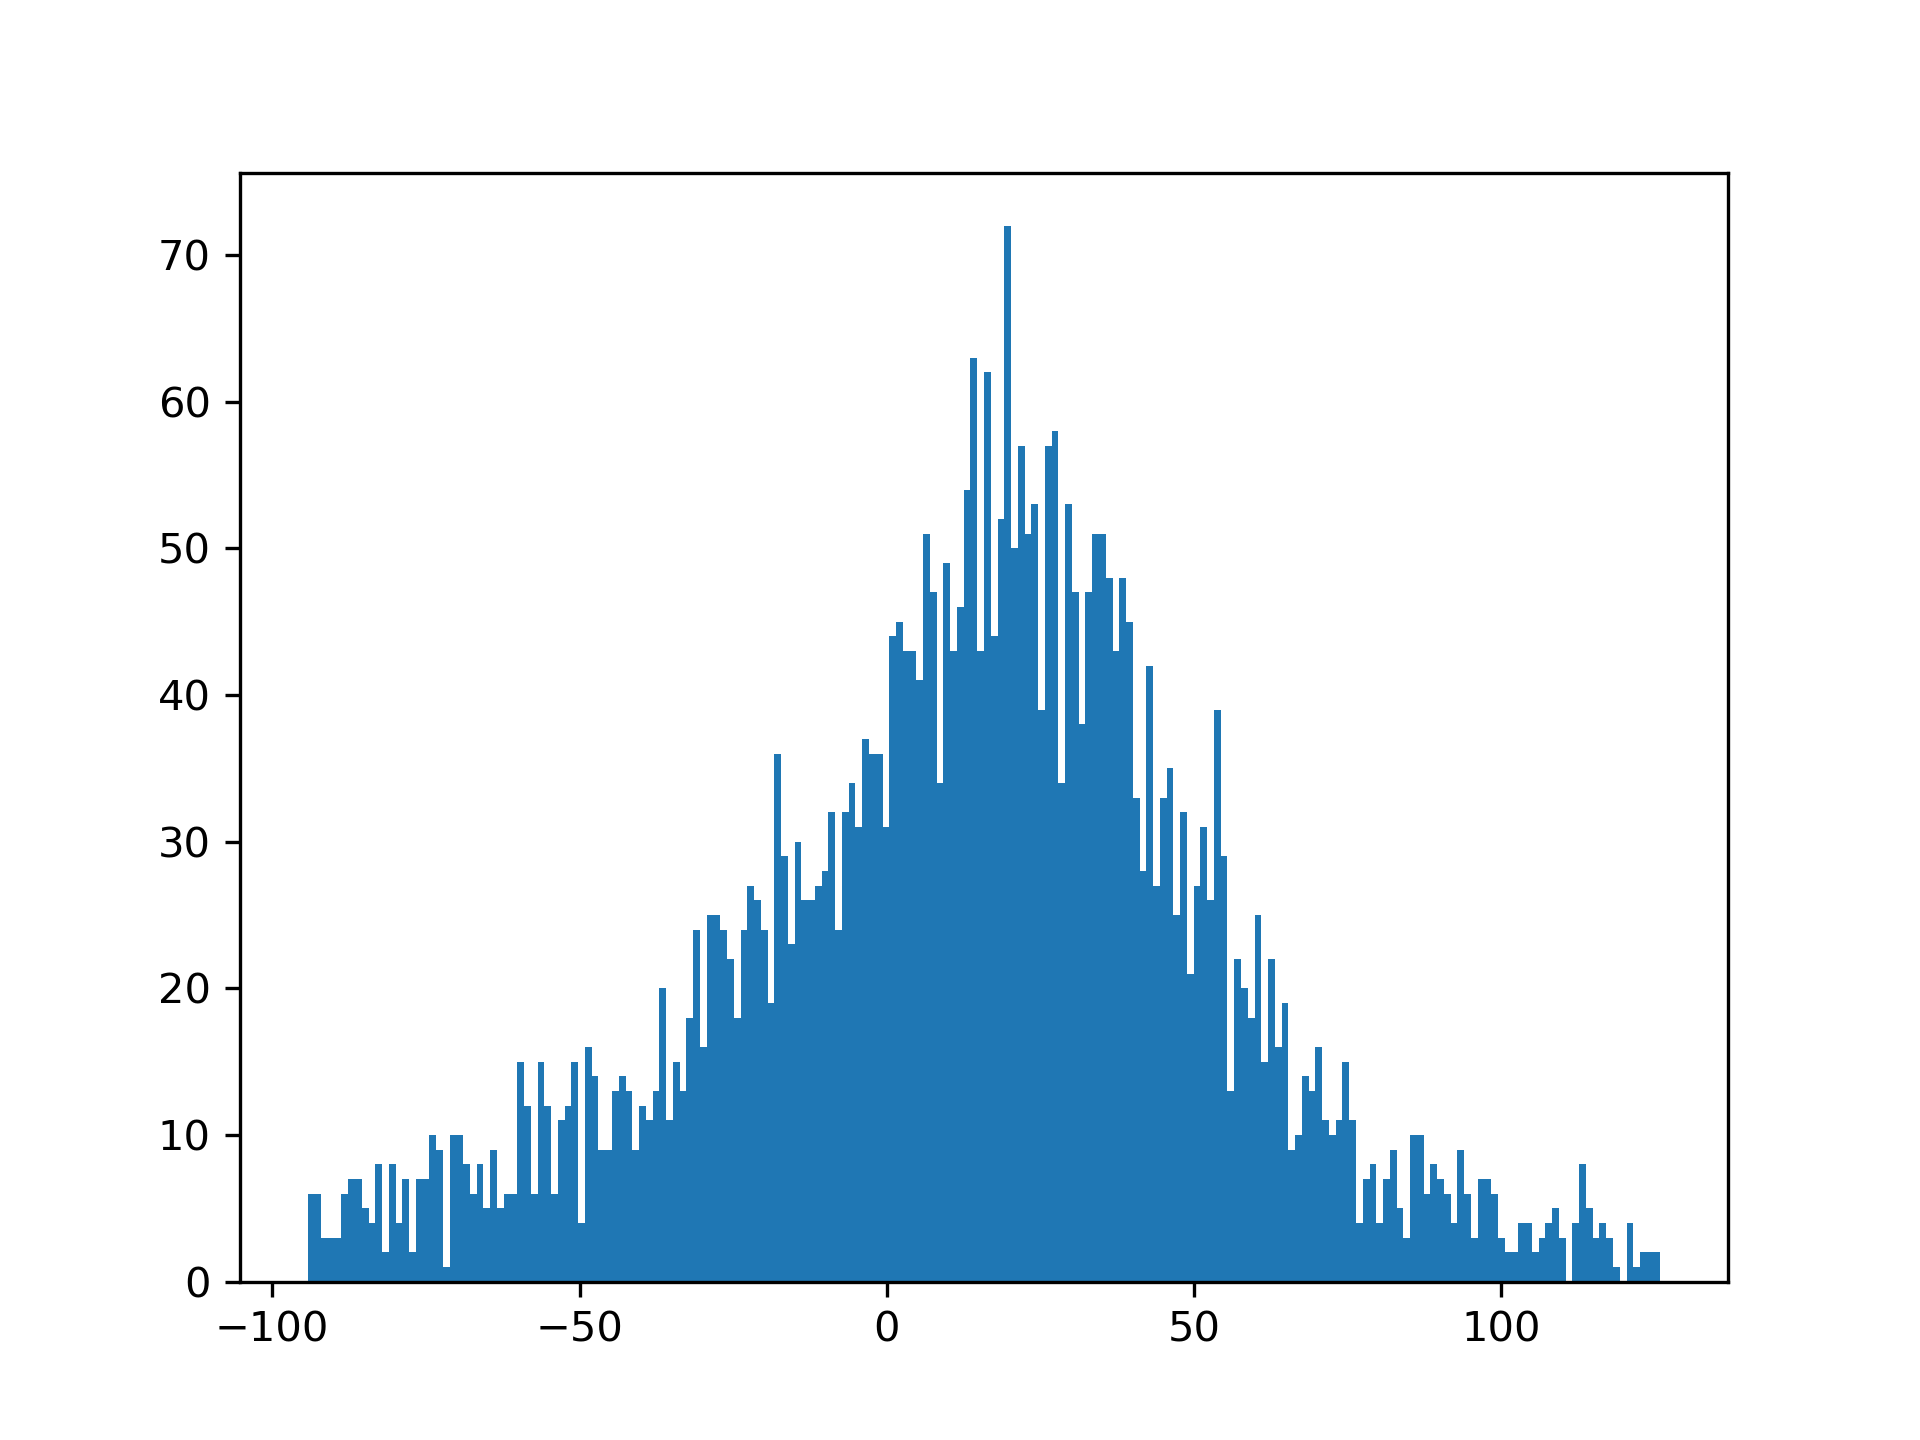
\includegraphics[width=\linewidth]{source/YHistogram.png}
    \caption{Histogram zmiennej objaśnianej}
\end{figure}

\newpage
\subsection{Korelacja}
Korelacja zmiennej objaśnianej ze zmiennymi objaśnianymi jest bardzo słaba, co osłabia możliwości prognostyczne modelu.
\begin{table}[h!]
    \begin{center}
    \begin{tabular}{|c | c|} 
    \hline
    Statystyka & Wartość \\
    \hline\hline
    Średnia arytmetyczna & 0.0006535276131026212 \\ 
    \hline
    Odchylenie standardowe & 0.01430737685985159 \\
    \hline
    Kwartyl dolny & -0.006560508005214499 \\
    \hline
    Mediana & 0.0009029552423272379 \\
    \hline
    Kwartyl górny & 0.008516164727314403 \\
    \hline
    Wartość najmniejsza & -0.07707504123521973 \\
    \hline
    Wartość największa & 0.04058496958769639 \\
    \hline
    \end{tabular}
    \end{center}
   \caption{Korelacja zmiennej objaśnianej ze zmiennymi objaśnianymi}
\end{table}

\begin{figure}[h!]
    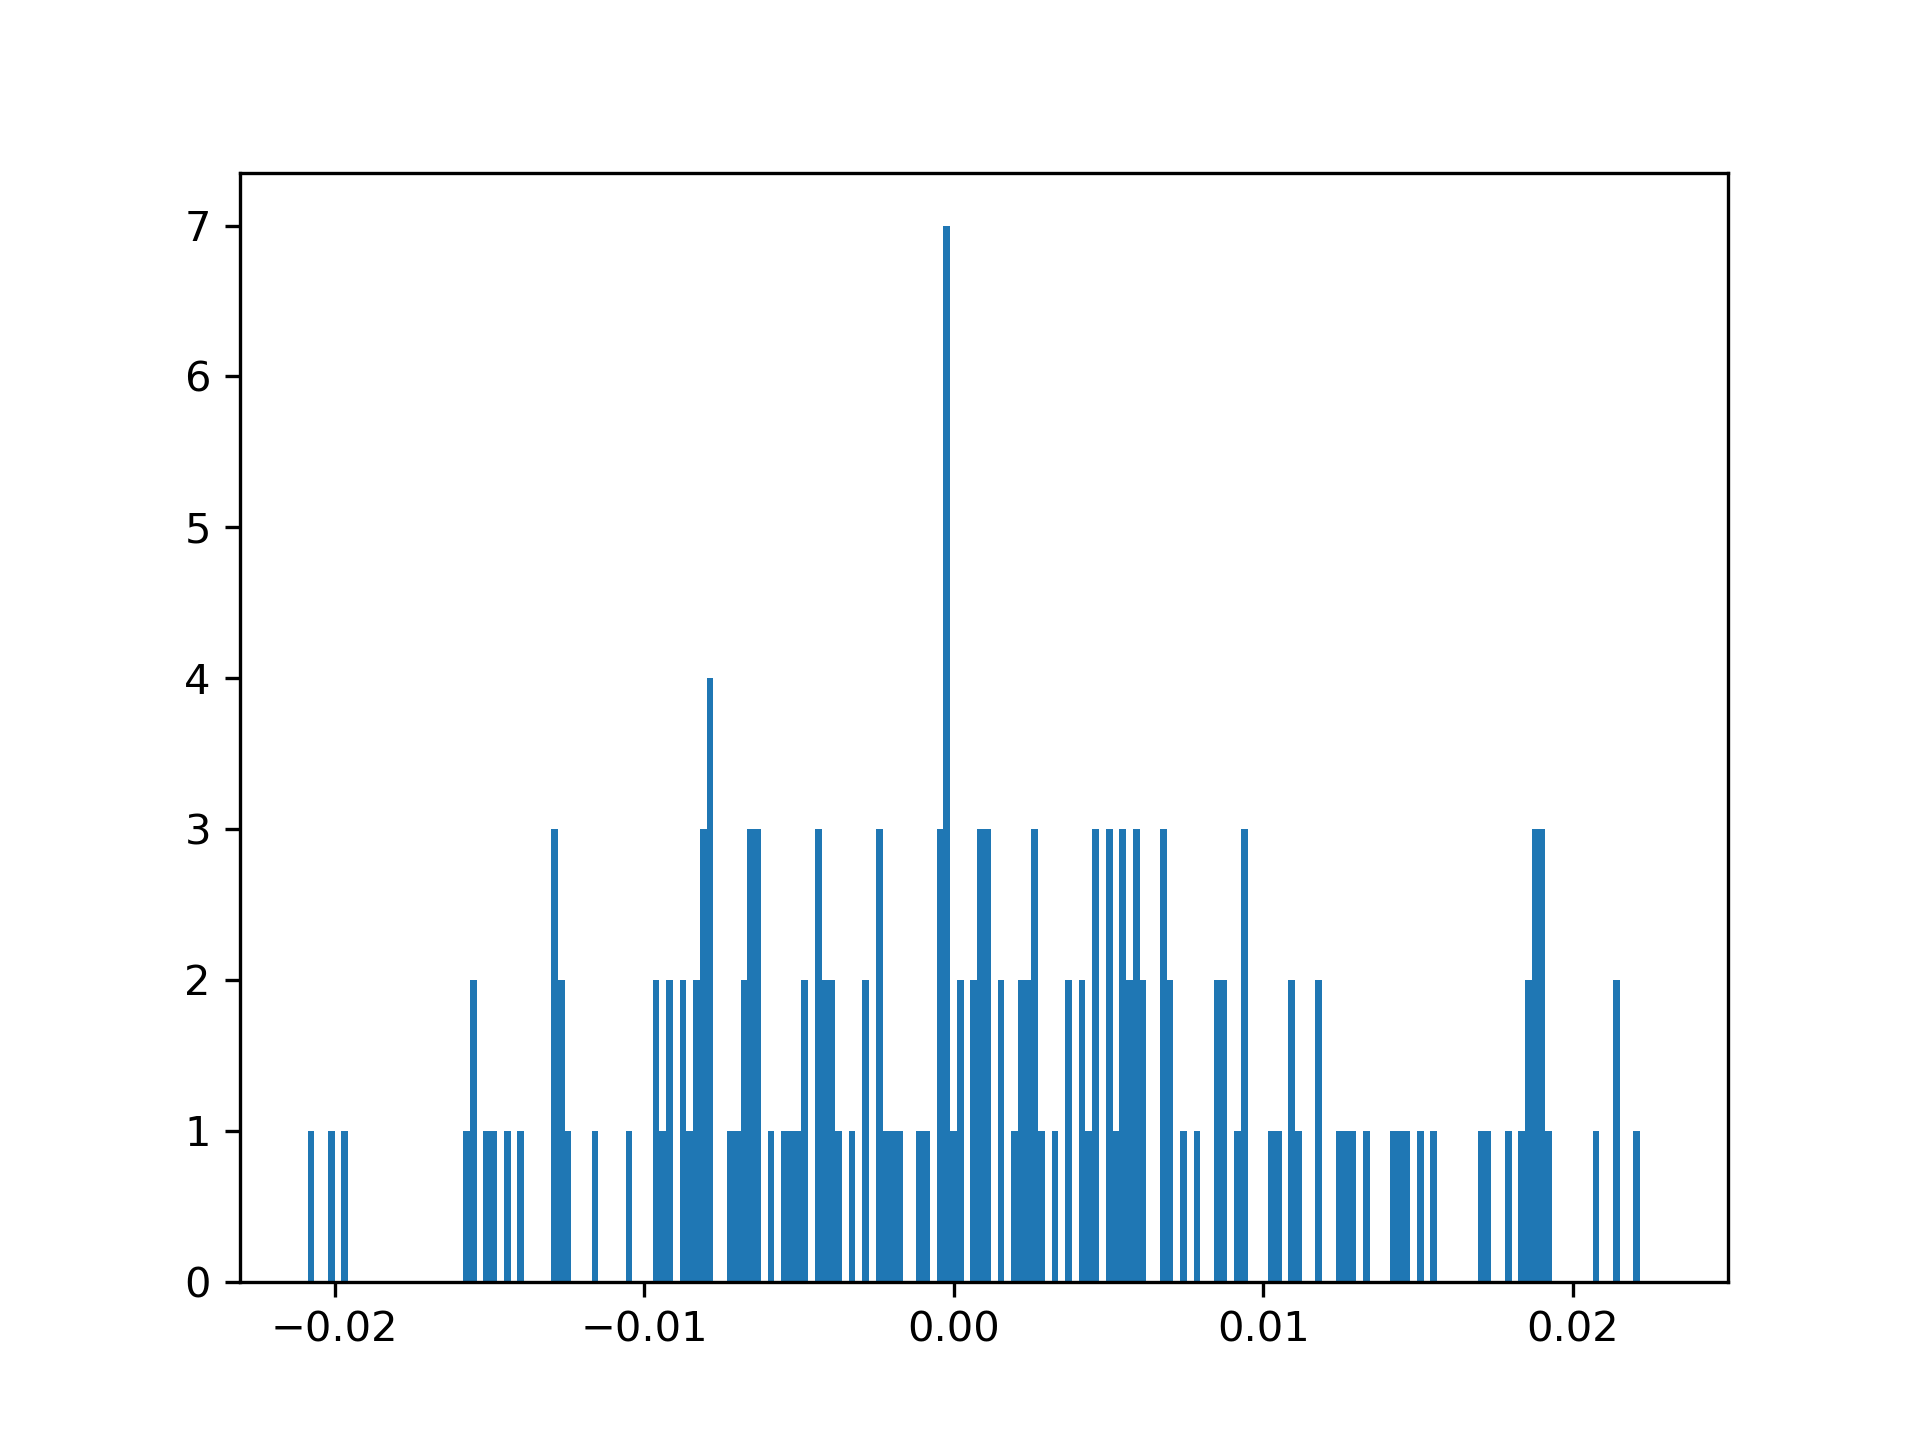
\includegraphics[width=\linewidth]{source/CorrHist.png}
    \caption{Histogram korelacji zmiennej objaśnianej ze zmiennymi objaśnianymi}
\end{figure}

\newpage
Korelacja pomiędzy niektórymi zmiennymi objaśniającymi jest silna, co można wyjaśnić zależnościami pomiędzy rozmiarem spółki, a wielkościami w \textit{10-K Form}. Nie wszystkie zmienne objaśniające mogą znaleźć się w modelu, ponieważ spowodowałoby to wystąpienie zjawiska współliniowości.
\begin{figure}[h!]
    \includegraphics[width=\linewidth]{source/CorrelationMatrix.png}
    \caption{Macierz korelacji}
\end{figure}

\newpage
\section{Dobór zmiennych do modelu}
fadsfda
\section{Wybór postaci modelu}

\section{Weryfikacja statystyczna modelu}

\section{Prognoza}

\section{Interpretacja}

\section{Podsumowanie}

\newpage
\section{Spis tabel}
\listoftables


\newpage
\section{Spis rysunków}
\listoffigures


\newpage
\section{Literatura}
\printbibliography

\end{document}
